%%## MASTER THESIS

%% DOCUMENTCLASS %%
%%\documentclass[11pt, DIV=calc, BCOR=10mm, twoside]{scrbook} 
\documentclass[a4paper,11pt,twoside,onecolumn,openright,final]{memoir} %scrartcl scrreprt scrbook %memoir

% Präambel für Master Thesis
% Dokumentenklasse
\documentclass[a4paper, 
                11pt, 
                twoside, 
                onecolumn, 
                openright,
                final]{memoir}

%% Pakete
% Unterscheidung zwischen compiler LuaLaTeX vs pdfLaTeX
\usepackage{ifluatex}
\ifluatex 
    % lualatex
    \usepackage{polyglossia}
    \setmainlanguage{german}
    \usepackage{fontspec}
    %\defaultfontfeatures{Ligatures=TeX}
    %\usepackage[]{unicode-math} 
    %\unimathsetup{math-style=TeX}
    \setmainfont[Ligatures=TeX]{DejaVuSerif} 
    \setsansfont{DejaVuSans}
    \setmonofont{DejaVuSansMono}
\else 
    % pdflatex
    \usepackage[T1]{fontenc}
    \usepackage[utf8]{inputenc}
    % Schriftarten
    \usepackage{palatino}       % Serifen %times
    \usepackage[scaled]{helvet} % Serifenlos
    \usepackage{courier}        % Schreibmaschinenschrift
    %\usepackage{mathptmx}      % Matheschrift
\fi

%% Sprache
%\usepackage[ngerman, british]{babel}


%% Allgemeines Layout
\setbinding{1cm} % bindekorrektur
% \semiisopage[] 
\semiisopage[9]
% \setlrmargins{*}{1cm}{*}
\OnehalfSpacing % zeilenabstand
\usepackage[document]{ragged2e} % linksbündig 
\usepackage[babel,german=quotes]{csquotes} % Anführungszeichen
\usepackage{color}                    % farbe 

%% Layout Kopf- und Fußzeile
% plain
\makeevenhead{plain}{}{}{}
\makeevenfoot{plain}{}{\thepage}{}
\makeoddhead{plain}{}{}{}
\makeoddfoot{plain}{}{\thepage}{}
% headings
\makeevenhead{headings}{\leftmark}{}{}
\makeevenfoot{headings}{}{\thepage}{}
\makeoddhead{headings}{}{}{\rightmark}
\makeoddfoot{headings}{}{\thepage}{}
% sep line
%\makeheadrule{plain}{\textwidth}{.5pt}
\makefootrule{plain}{\textwidth}{.5pt}{0ex}
\makeheadrule{headings}{\textwidth}{.5pt}
\makefootrule{headings}{\textwidth}{.5pt}{0ex}

%% Querverweise
\usepackage[linktoc=all, hypertexnames=false, plainpages=false, pdfpagelabels]{hyperref}
\usepackage{memhfixc}

%% Inhaltsverzeichnis
%\usepackage[nottoc,numbib]{tocbibind}
\setcounter{tocdepth}{1}

%% Matheumgebungen
\usepackage[fleqn]{mathtools}

%% SI-Einheiten
\usepackage{siunitx}
\sisetup{locale = DE,
          list-final-separator = \text{~und~},
          list-pair-separator = \text{~und~},
          range-phrase = \text{~bis~}}
\DeclareSIUnit\year{yr}
%\usepackage[german]{translator}

%% Abbildungen
\usepackage{tikz}
\usepackage{graphicx}
\usepackage{float} % für Fließumgebungen; Platzierung H verschiebt nicht
\restylefloat{figure}
\ifluatex
    \newcommand{\includegraphicstikz}{\input}
\else
    \newcommand{\includegraphicstikz}{\includegraphics}
\fi

%% Captions von Tabellen und Abbildungen
\makeatletter
\renewcommand{\fnum@table}[1]{\small \textbf{\tablename~\thetable:} }
\renewcommand{\fnum@figure}[1]{\small \textbf{\figurename~\thefigure:} }
\makeatother

%% Tabellen
% \usepackage{tabular}
\usepackage{tabularx}
\newcommand{\minitab}[2][l]{\begin{tabular}{#1}#2\end{tabular}}
\usepackage{multirow}
\usepackage{bigstrut}


%% Zitation und Literaturverzeichnis
\usepackage[square, semicolon]{natbib}
\bibliographystyle{abbrvnat} % plainnat abbrvnat unsrtnat
\usepackage{url}


%% Blindtexte
\usepackage{blindtext, lipsum}


%
%% ## Ende der Präambel



\begin{document}
\frontmatter

%% ## Titelseite
\begin{titlingpage}

\begin{center}%
%\vspace{1cm}
\begin{minipage}{0.45\textwidth} %0.49
  \begin{center}
  
\includegraphics[width=0.55\textwidth]{01-figures/c-logo_miub} \\
  \end{center}
\end{minipage} 
\hfill %
\begin{minipage}{0.45\textwidth} %0.49
  \begin{center}
  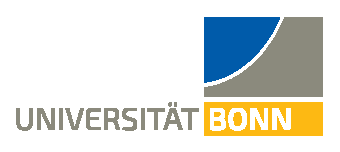
\includegraphics[width=0.7\textwidth]{01-figures/c-logo_uni_2017} \\
  \end{center}
\end{minipage}

\vspace{1cm} \hrule \vspace{1cm}

\begin{LARGE}
  Klimatologische Analyse der Jetstreams \\
  der oberen Troposphäre \\
  auf der nördlichen Hemisphäre \\
\end{LARGE}
\vspace{1cm} \hrule \vfill

\normalsize 
Masterarbeit\\im Studiengang\\
Physik der Erde und Atmosphäre
     
\vfill
Rheinische Friedrich-Wilhelms-Universität Bonn\\
Mathematisch-Naturwissenschaftliche Fakultät\\
Meteorologisches Institut\\

\vfill
\textbf{Sebastian Kiefer} \\ % \vfill
Bonn im September 2017
\end{center}
\end{titlingpage}

\thispagestyle{empty}
%\quad
%\newpage
%\thispagestyle{empty}
\begin{center}
\begin{tabular}{ l l }
Betreuer der Masterthesis: & \textbf{Prof. Dr. Andreas Hense} \\
\\
%& (Meteorologisches Institut der Universität Bonn) \\
Gutachter der Masterthesis: & \textbf{Prof. Dr. Andreas Bott} \\
%& (Meteorologisches Institut der Universität Bonn) \\
& \textbf{PD Dr. Petra Friederichs} \\
%& (Meteorologisches Institut der Universität Bonn) \\
\end{tabular}
\end{center}


\vspace*{\fill}
\large{\textbf{\underline{Eigenständigkeitserklärung}}}
\normalsize

\vskip 1cm

\noindent
Hiermit versichere ich, dass ich die vorliegende Arbeit selbstständig verfasst und keine anderen als die angegebenen Quellen und Hilfsmittel benutzt habe, dass alle Stellen der Arbeit, die wörtlich oder sinngemäß aus anderen Quellen übernommen wurden, als solche kenntlich gemacht sind und dass die Arbeit weder in gleicher noch in ähnlicher Form noch keiner Prüfungsbehörde vorgelegt wurde.

\vskip 2cm

\parbox{5.5cm}{\centering Bonn, \today
{\hrule height .5pt}
\strut \centering\footnotesize Ort, Datum} \hfill
\parbox{5.5cm}{\centering \textcolor{white}{\centering Bonn, \today} 
{\hrule height.5pt}
\strut \centering\footnotesize Sebastian Kiefer}
 


\newpage
\thispagestyle{empty}
\quad
\newpage
\thispagestyle{empty}
\tableofcontents  % Inhaltsverzeichnis
\listoffigures    % Abbildungsverzeichnis
%\listoftables    % Tabellenverzeichnis
\newpage

\mainmatter %% ## 

% \begin{abstract} % scrreprt
% \blindtext
% \end{abstract}

\chapter*{}
\addcontentsline{toc}{chapter}{Abstract \& Zusammenfassung}


\begin{center} \begin{bfseries}
  Abstract
\end{bfseries} \end{center}

\begin{quotation}
  \blindtext
\end{quotation}


\begin{center} \begin{bfseries}
  Zusammenfassung
\end{bfseries} \end{center}

\begin{quotation}
  \blindtext
\end{quotation}


\part{Einleitung}
\chapter{Motivation und Zielsetzung} \label{ch:motivation}

Der Klimawandel ist weltweit allgegenwärtig \citep{ipcc-2014}. Die Auswirkungen der globalen Erwärmung zeigen sich in schmelzenden Gletschern, steigenden Meeresspiegeln, Extremwetterereignissen wie Dürren und Überschwemmungen, im Monsun und in tropischen Zyklonen. Diese Auswirkungen und besonders die damit verbundenen Risiken, die sich aus der Vulnerabilitt und der Exposition gegenüber Gefahren durch natürliche Variabilität und anthropogene Klimaänderungen zusammensetzen, sind global ungleich verteilt. So sind Dürren in ohnehin trockenen Regionen wie im mittleren Osten besonders spürbar \citep{ipcc-wg2-2014}. In Syrien ist eine mehrjährige Dürreperiode einer der Auslöser für den seit 2011 anhaltenden Bürgerkrieg und die Flucht der Menschen in den Libanon und nach Europa gewesen \citep{gleick-2014}.  

Die Ursache für den globalen Temperaturanstieg sind in die Atmosphäre ausgestoßene Treibhausgase wie Kohlenstoffdioxid CO$_2$ und Methan CH$_4$, der Klimawandel ist hauptsächlich menschengemacht \citep{ipcc-wg1-2013}. So wurden seit 1850 rund $1000$\,Gto\,CO$_2$ maßgeblich von den Industrienationen emittiert. Seitdem die Industrialisierung in den Schwellenländern Einzug gehalten hat, steigt deren Beitrag am globalen CO$_2$-Ausstoß besonders seit 2000 rasant an. Genannt seien hier insbesondere die BRICS-Staaten, die in Absolutbeträgen die Liste der Emittenten bereits anführen, auf die Einwohnerzahl normiert jedoch deutlich hinter die Industriestaaten zurückfallen. \citep{ipcc-wg3-2014}

Dies offenbart eine enorme Diskrepanz, da die Industriestaaten, die historisch die Hauptemittenten von Treibhausgasen sind, die Auswirkungen des eigenen Handelns lediglich indirekt zu spüren bekommen. Schlimmer, auch wenn Auswirkungen spürbar sind wie in erhöhter Zuwanderung aus der MENA-Region in Süd- und Zentraleuropa, Sturmfluten in den Niederlanden oder tropischen Wirbelstürmen in den Vereinigten Staaten von Amerika, wird dies nur selten als Handlungsaufforderung zur Minderung der Treibhausgas-Emissionen begriffen. Statt die Wirtschaft auf eine nachhaltige Spur zu bringen, werden Anpassungs- und Abschottungsmaßnahmen ergriffen. In Deutschland rücken wirksame Maßnahmen zur Minderung in weite Ferne. Die Energiewende stagniert, nach einer Wende im Verkehrssektor lässt sich lange suchen und am Paradigma des ewigwährenden Wirtschaftswachtums wird weiter festgehalten. 

Um zu ergründen, welcher Natur die großräumigen Auswirkungen des Klimawandels in den mittleren Breiten sind, wird in dieser Arbeit ein Wetterphänomen untersucht, dass für eben diese Regionen wetterbestimmend ist. Als eines, zu dem auch schon geforscht wird, sei an dieser Stelle der Polarfront-Jetstream benannt. Der Jetstream (oder auch Strahlstrom) wird von der Weltorganisation für Meteorologie definiert als ein starke schmale Strömung, die sich entlang einer horizontalen Achse durch eine starke horizontale und vertikale Windscherung auszeichnet \citep{wmo-1958}. Dieser mäandriert in Wellenform um den Nordpol, wobei die Welle selbst ostwärts propagiert. In den vergangenen Jahren hat es ein paar Male die Situation gegeben, dass der polare Jetstream über einen längeren Zeitraum seine Position nicht verändert hat, die Welle also nicht wie üblich propagierte. Diese Stagnation führte beispielsweise im Winter 2013/14 zu Rekordschneefällen an der Ostküste der Vereinigten Staaten von Amerika \citep{palmer-2014} und im Sommer 2003 zu einer Hitzewelle in Westeuropa \citep{petoukhov-2013}.

In den Klimawissenschaften herrscht Einigkeit darüber, dass ein Anstieg der globalen Temperatur mit hoher Wahrscheinlichkeit zu einem vermehrten Auftreten von Rekordtemperaturen. Ebenso erhöht sich der atmosphärische wassergehalt, was die Wahrscheinlichkeit von Starkregenereignissen erhöht. Die steigenden Temperaturen auf der Landfläche sorgen für eine höhere Verdunstung, was die Landwirtschaft änfälliger gegenüber Dürren macht. Während die Atmosphäre und der Ozean erwärmt, dehnt sich Meerwasser aus und Gletscher und Eisschilde schmelzen. Hierdurch steigt der Meeresspiegel. Verglichen mit diesen Wirkungsketten erscheint der hergestellte Zusammenhang zwischen einer Abnahme arktischen Seeeises und einem kälteren Winter in den Vereinigten Staaten zunächst kontraintuitiv. \citep{wallace-2014}

Über Änderungen in der globalen Zirkulation ließe sich auch in einem wärmeren Klima, das grundsätzlich die Wahrscheinlichkeit für kalte Winter mindert, das häufigere Auftreten kalter Winter erklären. Klimatologische Veränderungen in der Häufigkeit unterschiedlicher Zirkulationsmuster manifestieren sich einer Veränderung der Position der Jetstreams. Der polare Jetstream der nördlichen Hemisphäre führt Luftmassen über Rossby-Wellen von West nach Ost. Über diese Wellen werden kalte Luftmassen südwärts und umgekehrt warme Luftmassen nordwärts transportiert, sodass Regionen, die unter einem nach Süden führenden Jet liegen, wahrscheinlich kälteres Wetter zu spüren bekommen, während für Regionen, die unter einem nach Norden führenden Jet liegen, der umgekehrte Fall gilt. Sie erfahren wärmeres  Wetter. \citep{palmer-2014}

Um langfristige Veränderungen des Jetstreams zu erkennen, werden in dieser Arbeit zwei unabhängige Methoden zur Detektion von Jetstreams und zur Differenzierung zwischen Polarfront- und subtropischem Jetstream auf einen Datensatz, der aus ERA-Interim- und ERA-40-Daten von 1957 bis 2017 besteht, angewandt und die Positionen der Jetstreams sowie deren Zonal- und Meridionalwindgeschwindigkeiten auf Veränderungen in Zeit und Raum untersucht. Dies geschieht sowohl auf jährlichen als auch auf saisonalen Skalen. Darüber hinaus wird der Zusammenhang zwischen der arktischen Amplifikation und den Veränderungen des Polarfrontjets analysiert.

\section*{Gliederung}
Gegliedert ist die Arbeit hierbei in folgende Abschnitte: Aufbauend auf der Motivation wird in Kapitel \ref{ch:hintergrund} der Stand der Forschung präsentiert und eingeordnet. Darauffolgend (Kap. \ref{ch:methodik}) werden die genutzten Datensätze sowie die beiden verwendeten Methoden zur Detektion von Jetstreams vorgestellt. In Kapitel \ref{ch:plausibilitaet} wird die Plausibilität der berechneten Jetstreampositionen zunächst anhand von zufällig ausgewählten Einzelfallbeispielen untersucht, bevor die beiden Methoden miteinander verglichen werden. Die zeitliche und raumzeitliche Analyse der Ergebnisse findet in Kapitel \ref{ch:klimatologie} statt, in dem Trends der Positionen und Windgeschwindigkeiten ebenso wie die Entwicklung der Variabilität untersucht werden. In Kapitel \ref{ch:seeeis} wird untersucht, ob ein Zusammenhang zwischen der Ausdehnung des arktischen Seeeises und der Position des Polarfrontjetstreams und dessen Variabilität besteht. Zu guter Letzt werden die Ergebnisse kurz diskutiert sowie ein Fazit gezogen.


\part{Hintergründe und Methodik}
\chapter{Stand der Forschung} \label{ch:hintergrund}

In diesem Kapitel wird der Stand der Forschung vorgestellt. Zu Veränderungen der großräumigen Zirkulation und insbesondere zu veränderten Wettermustern in den mittleren Breiten wird bereits geforscht. Daher wird an dieser Stelle eine knappe Historie wegweisender Forschungsarbeiten der vergangenen Jahre gegeben.

\citet{francis-2012} beschäftigen sich mit der Frage, wie die großräumige atmosphärische Zirkulation von der im Winterhalbjahr vom Ozean abgegebenen Wärme beeinflusst wird, die durch die Aufnahme solarer Strahlung von größer werdenden Freiwasserflächen zunimmt. Diese Fragestellung baut auf Arbeiten aus 2009 und 2010 auf, die herausgearbeitet haben, dass sich die bodennahen Luftschichten sowie der obere Teil der Arktis etwa doppelt so schnell erwärmt wie die gesamte nördliche Hemisphäre. Einzelne Extremwettereignisse haben zwar typischerweise einen dynamischen Ursprung, resultieren jedoch aus anhaltenden Zirkulationsmustern, die häufig mit blockierenden Rossbywellen mit hohen Amplituden verbunden sind. Als Beispiele hierfür werden die Hitzewellen 2010 in Europa und Russland, die Überschwemmungen am Mississippi 1993 und die Kälteereignisse in Florida im Winter 2010/11 genannt. 
Die Analyse unterstützt zwei Hypothesen, nach denen die arktische Amplifikation zu anhaltenden Zirkulationsmustern führen kann, die wiederum in Extremwetterereignissen resultieren können. Eine Ursache ist der schwächere meridionale Gradient der \SIrange{1000}{500}{\hecto\pascal}-Schichtdicke, was die Rossby-Welle auf eine nördlichere Amplitudenbahn drängt und so zu langsameren Zirkulationssystemen führt. Dies erhöht die Wahrscheinlichkeit für Extremwetterereignisse, die von persistenten Wetterlagen verursacht werden. Die zweite Ursache ist eine nordwärts gerichtete Verlagerung der Rücken der Wellen im \SI{500}{\hecto\pascal}-Druckniveau, was zu einer höheren Amplitude der Strömung führt und die Wahrscheinlichkeit von Blocking-Situationen weiter erhöht. Die Studie schließt damit, dass durch das weitere Schwinden der arktischen Meereisbedeckung davon auszugehen ist, dass die großräumige Zirkulation zunehmend durch die arktische Amplifikation beeinflusst wird.

Ziel von \citet{screen-2013} ist, die atmosphärischen Veränderungen besser zu verstehen, die möglicherweise als Reaktion auf die beobachteten Rückgänge des arktischen Meereises in den letzten drei Jahrzehnten eingetreten sind. Die Ergebnisse aus Simulationen mit zwei unabhängigen allgemeinen generellen Zirkulationsmodellen, deren einziger Antrieb die Variationen der Beobachtungen des arktischen Meereises zwischen 1979 und 2009 waren, deuten darauf hin, dass atmosphärische Auswirkungen auf den Verlust des Meereises am stärksten innerhalb der maritimen und Küstenregionen der Arktis auftreten. Die Modelle legen nahe, dass die Abnahme des arktischen Meereises den Energietransfer vom Ozean in die Atmosphäre, die verstärkte Erwärmung und die zunehmende Feuchte der unteren Troposphäre, die Stärke der Inversion sowie die erhöhte Schichtdicke der unteren Troposphäre beeinflusst. Die Modelle zeigen kaum Anzeichen für eine durch das Meereis hervorgerufene Temperaturänderung oberhalb der stabilen Grenzschicht, obwohl Beobachtungen und Analysen bereits auf eine Temperaturerhöhung hindeuten. Die beobachtete arktische Erwärmung in der Höhe wird wahrscheinlich durch Änderungen der Oberflächentemperatur des Meeres und die resultierende Zunahme des polumschlagenden Wärmetransports in die Arktis verursacht. Die Modellexperimente ermöglichen die Isolierung von durch Meereis verursachten atmosphärischen Veränderungen, die sich sowohl in gekoppelten Modellversuchen als auch in der Natur nur schwer entschlüsseln lassen. Die Analyse verschiedener Kälteperioden der vergangenen Jahre hat gezeigt, dass die Modelle keine robuste und weit verbreitete Abkühlung und keine erhöhten Schneefälle als Antwort auf die arktische Amplifikation in den letzten drei Jahrzehnten simulieren. Dies schließt zwar nicht aus, dass in den Wintern 2009/10 und 2010/11 die Meereisbedingungen eine treibende Rolle spielten, aber es deutet darauf hin, dass die vorgeschlagenen Verbindungen zwischen multidekadalen Änderungen des Meereises und der borealen Winterkühlung möglicherweise verfrüht sind.

\citet{petoukhov-2013} haben sich mit der quasiresonanten Amplifikation von planetaren Wellen und Wetterextrema der nördlichen Hemisphären auseinandergesetzt. Im Nachgang des außergewöhnlichen Sommers in 2003 in Europa wurde vorgeschlagen, dass der beobachtete Klimatrend die Wahrscheinlichkeitsverteilung der Sommertemperaturen in Richtung wärmerer Werte verschiebt und diese Verteilung verbreitert, sodass Extremwerte wahrscheinlicher werden. Jedoch erklärt auch eine veränderte Wahrscheinlichkeitsverteilung die regionalen Sommerextrema der vergangenen Jahre nicht vollständig, sodass angenommen wird, dass kein rein stochastischer Extremwirkungsmechanismus am Werk ist. Die Hitzewellen in Russland in 2010 sowie in den Vereinigten Staaten in 2011, deren Muster sich räumlich über die gesamte Hemisphäre und zeitlich über den gesamten Sommer erstreckten, legen nahe, dass es sich nicht um typische Blocking-Lagen mit einer charakteristischen Zeit von fünf bis sieben Tagen handelt. Eine quasistationäre freie synoptisch-skalige Welle schwingt quasiresonant, sobald die beiden so genannten Wendepunkte der mittleren Breiten für die Welle auftreten, sodass eine starke dynamische Reaktion auf die klimatologischen diabatischen und orographischen Antriebe begünstigt wird. Die vorliegenden Daten und Ergebnisse deuten auf eine Veränderung der atmosphärischen Bedingungen hin, sodass die betrachtete quasiresonante Amplifikation häufiger auftreten könnte.

In \citet{barnes-2013-b} wird im CMIP5-Modell (Coupled-Model-Inter\-com\-parison-Project Phase 5) untersucht, wie Jetstreams über den mittleren Breiten auf eine Zunahme der CO$_2$-Konzentration in der Atmosphäre reagieren. In allen untersuchten Regionen (Nordatlantik, Nordpazifik und südliche Hemisphäre) zeigen die Analysen eine Verschiebung der Jetstreams in Richtung der Pole um etwa \SIrange{1}{2}{\degree} zum Ende des 21. Jahrhunderts. Darüber hinaus verändert sich die Variabilität. So wird für den Nordatlantik ein eher pulsierender und weniger mäandrierender Jet prognostiziert, während für den Nordpazifik der umgekehrte Fall gilt. Da einige Projektionen starke Veränderungen in der Jetposition simulieren, halten \citet{barnes-2013-b} es für möglich, dass sich das Variabilitätsmuster in Zukunft deutlich vom bekannten Verhalten der Jetstreams unterscheidet. Die Jetstreamvaribilität ist stark verbunden mit den Zugbahnen von Tiefdruckgebieten, dem regionalem Wetter sowie mit Blockings von Hochdruckgebieten. Durch diese vielfältigen Verbindungen zu physikalischen Prozessen in der Troposphäre und der Erdoberfläche werden Veränderungen in den dominanten Variabilitätsformen der Jetstreams wichtige globale Auswirkungen haben.

\citet{barnes-2013-a} quantifiziert beobachtete Trends der meridionalen Ausdehnung von Wellen über dem Nordatlantik und -amerika mit Hilfe von zwei verschiedenen Maßen und drei Reanalysen. Die Maße zeigen nicht übereinstimmend, ob ein signifikanter Trend der Veränderungen der Wellenamplituden beobachtet wird. Die Uneinigkeit entstammt der Autorin zufolge den unterschiedlichen Methoden, die Wellen entweder auf täglichen oder auf saisonalen Zeitskalen definieren. Verlangsamt haben sich großskalige Wellen in den vergangenen Jahrzenten lediglich in den Herbstmonaten signifikant, wobei die Signifikanz des Trends sensibel auf Änderungen der Region reagiert. Darüber hinaus ist zu keiner Jahreszeit ein signifikanter Anstieg des Auftretens von Blockings festzustellen. Sie kommt zu dem Schluss, dass die Hypothese, dass eine verstärkte polare Erwärmung zu einem vermehrten Auftreten von sich langsam verlagernden Wettermustern führt, nicht durch Beobachtungen gestützt wird. Die Arktis verändere sich rasant und diese Veränderungen werden voraussichtlich tiefgreifende Auswirkungen auf die nördliche Hemisphäre haben. Diese Studie zeigt jedoch, dass die Beziehung zwischen der arktischen Amplifikation und dem Wetter der mittleren Breiten komplex ist. Zusätzliche Einflüsse aus anderen Breitengraden sowie interne Variabilität spielen wahrscheinlich eine wichtige Rolle bei der Bestimmung der atmosphärischen Trends und gezielte Modellierungsstudien seien notwendig, um die relative Bedeutung der Polarveränderungen auf das atlantische Wetter zu quantifizieren.

Aufbauend auf Arbeiten aus 2012 und 2013, die zeigen, dass die Erwärmung der Arktis und die Abnahme von polarem Meereis zu einer Zunahme von Blockings auf der nördlichen Hemisphäre geführt haben, untersuchen \citet{barnes-2014}, ob die Häufigkeit solcher Blockings in den letzten Jahrzehnten robuste Trends aufweisen. Dies wird mit wird mit drei Methoden in vier Reanalysen untersucht. Für den Blocking-Index ist zu keiner Jahreszeit eine deutliche Zunahme von Blockings festzustellen, obwohl einzelne Regionen und Jahreszeiten robuste Unterschiede zeigen. Vergleiche der Blockingfrequenzen im September zwischen Jahren mit einer starken Ausdehnung des Seeeises und jenen mit einer geringen Seeeisausdehnung zeigen deutliche Unterschiede. In den Sommermonaten zeigen sich positive Differenzen über dem Nordatlantik und Negative über dem Nordpazifik. Es wird davor gewarnt, die Ergebnisse schlicht als Nachweis von Blockings als Antwort auf Seeeisverluste zu interpretieren. Die Veränderungen können vielmehr von einer Vielzahl unterschiedlicher dynamischer Mechanismen ausgelöst werden. Insgesamt stützen diese Schlussfolgerungen die Untersuchungen von \citet{barnes-2013-a}, dass der Zusammenhang zwischen der arktischen Amplifikation und häufigeren Blockadesituationen auf der nördlichen Hemisphäre derzeit nicht durch Beobachtungen gestützt wird. Während das arktische Meereis in den vergangenen Jahren nie da gewesene Verluste verzeichnet, scheinen Blockings nicht außergewöhnlich und liegen innerhalb der historisch beobachteten Größenordnung. Die große Variabilität der Blocking-Ereignisse, sowohl auf interannualer als auch auf dekadischer Zeitskala, zeigt die Schwierigkeit, eine potenziell durch den Klimawandel induzierte Reaktion von der natürlichen Variabilität zu unterscheiden.

\citet{cohen-2014} haben sich in einem Review-Artikel mit der arktischen Amplifikation und Extremwetter in den mittleren Breiten beschäftigt. Die rapide Erwärmung der Arktis hat zu einem dramatischen Abschmelzen des arktischen Meereises und der Schneedecke im Frühjahr geführt, und zwar in einem höheren als durch Klimamodelle simulierten Tempo. Diese tiefgreifenden Veränderungen des arktischen Systems sind mit einer Periode von vermeintlich häufiger auftretenden extremen Wetterereignissen in den mittleren Breitengraden der nördlichen Hemisphäre zusammengefallen. Die Möglichkeit eines Zusammenhangs zwischen dem arktischem Wandel und dem Wetter der mittlerem Breiten hat Forschungsaktivitäten angestoßen, die drei mögliche dynamische Wege aufzeigen, die die arktische Amplifikation mit den mittleren Breiten verbinden: Veränderungen der Zugbahnen von Tiefdruckgebieten, des Jetstreams und der planetaren Wellen. Durch die Veränderung dieser atmosphärischen Schlüsselmerkmale ist es prinzipiell möglich, dass Meereis und Schneedecke gemeinsam das Wetter in den mittleren Breiten beeinflussen. Aufgrund unvollständiger Kenntnisse über den Einfluss des Klimawandels auf diese Phänomene, kombiniert mit spärlichen und kurzen Datensätzen und unvollkommenen Modellen, bleiben jedoch große Unsicherheiten über die Größenordnung eines solchen Einflusses bestehen. \citet{cohen-2014} kommen zu dem Schluss, dass ein verbessertes Prozessverständnis, anhaltende und zusätzliche arktische Beobachtungen und besser koordinierte Modellierungsstudien erforderlich sind, um das Verständnis für Einflüsse auf das Wetter in den mittleren Breiten und dortige Extremereignisse zu verbessern.
Ein fundamentaler Treiber des Polarfrontjets ist der Temperaturunterschied zwischen der Arktis und den mittleren Breitengraden. Daher könnte eine niedrigere Temperaturdifferenz zu einer schwächeren Zonalwindkomponente und größeren Mäandern führen. Eine schwächere und mäandrierende Strömung kann dazu führen, dass die Wettersysteme langsamer nach Osten wandern, sodass persistente Wettermuster häufiger werden. Darüber hinaus führt die arktische Verstärkung dazu, dass die Schichtdicke der Atmosphäre nach Norden zunimmt, sodass sich die atmosphärischen Rücken nach Norden verlängern und somit die Amplituden der Strömung vergrößern können. Wetterextreme treten häufig auf, wenn die atmosphärischen Zirkulationsmuster anhaltend sind, was bei einer starken meridionalen Windkomponente tendenziell der Fall ist.
Einige Aspekte dieser hypothetischen Verknüpfung werden durch Beobachtungen und Modellsimulationen unterstützt. Ein signifikanter Rückgang des mittleren Zonalwinds bei \SI{500}{\hecto\pascal} im Herbst wird regional beobachtet. Dies lässt sich an der thermischen Windbeziehung ablesen, die besagt, dass die vertikale Windscherung proportional zum meridionalen Temperaturgradienten ist. Unter der Annahme, dass die Winde an der Oberfläche nicht zunehmen, sollte der zonale Wind auf Jetstream-Niveau mit einem schwächeren meridionalen Temperaturgefälle nachlassen. In anderen Jahreszeiten, in denen die arktische Amplifikation schwächer ist, ist kein signifikanter Trend des mittleren Zonalwinds zu beobachten.
Die Herausforderung bestehe jedoch weiterhin darin, die arktische Amplifikation direkt mit Änderungen der Geschwindigkeit und Struktur des Strahlstroms zu verknüpfen. Beispielsweise beeinflussen neben dem oberflächennahen meridionalen Temperaturgradienten weitere Faktoren den Jetstream, darunter die Rückkopplungen von synoptischen Eddies und Stürmen sowie der meridionale Temperaturgradient der oberen Tro\-po\-sphä\-re. Obwohl die arktische Verstärkung den oberflächennahen meridionalen Temperaturgradienten geschwächt hat, hat sich der Temperaturgradient zwischen den Tropen und den mittleren Breiten in der Höhe verstärkt, was zu einem Anstieg der Winde auf Jetstream-Niveau führen würde. Eine weitere Herausforderung besteht darin, herauszufinden, ob und wie groß der Anteil entfernter Veränderungen auf die arktische Amplifikation ist. Diese Unterscheidung ist von großer Bedeutung, denn wenn ein erheblicher Anteil aus der Ferne getrieben wird, kann die arktische Amplifikation teilweise eher als Reaktion auf das Wetter der mittleren Breiten und weniger als dessen Antrieb betrachtet werden.

Nach \citet{francis-2015} verschärft sich der Klimawandel in der Arktis weiter, das Schwinden des arktischen Meereises hält an und die Masse des grönländischen Inlandeises nimmt ab, die Schneebedeckung der nördlichen Hemisphäre während des Frühsommers geht zurück und die arktische Amplifikation hält weiter an. Der überproportionale Temperaturanstieg beeinflusst die großräumige Zirkulation möglicherweise mit weitreichenden Auswirkungen. Der NOAA-tabulated-climate-extreme-index \citep{karl-1996} hat in den Vereinigten Staaten im Vergleich mit den Jahren vor der arktischen Amplifikation um etwa ein Drittel zugenommen. Noch ist unklar, ob die Erwärmung der Arktis hierfür eine Ursache ist. \citet{francis-2015} weisen nach, dass in Regionen und Jahreszeiten, in denen sich die meridionalen Gradienten als Reaktion auf die Arktis abgeschwächt haben, der Fluss der oberen Troposphäre meridionaler oder welliger geworden ist. Darüber hinaus hat in den letzten Jahren die Häufigkeit von Tagen mit  Jetstreams mit hoher Amplitude zugenommen. Diese Muster, die sich durch hohe Amplituden auszeichnen, sind dafür bekannt, dass sie anhaltende Zirkulationsmuster erzeugen, die zu extremen Wetterereignissen führen können. Als Beispiele werden die kalten, schneereichen Winter im Osten der Vereinigten Staaten in den Wintern 2009/10, 2010/11 und 2013/14, die Rekordschneefälle in Japan und im Südosten Alaskas im Winter 2011/12 sowie die Überschwemmungen im Mittleren Osten im Winter 2012/2013 angeführt. Auf der Grundlage dieser Ergebnisse kommen sie zu dem Schluss, dass ein Fortschreiten der arktischen Amplifikation zu allen Jahreszeiten infolge des ungebremsten Anstiegs der Treibhausgasemissionen zu einem zunehmend welligen Charakter der Jetstreams der hohen Troposphäre und damit zu einer Zunahme extremer Wetterereignisse beitragen wird.

\citet{rikus-2015} hat ein einfaches Detektionsschema über geschlossene Konturlinien für den meridional und monatlich gemittelten Zonalwind entwickelt, um Jetstreams zu identifizieren, und auf \num{9} Reanalysedatensätze von \numrange{1979}{2009} angewandt. Um vermeintliche Jets zu lokalisieren, wird das über alle Meridiane und monatlich gemittelte Zonalwindfeld als zweidimensionales Bild betrachtet. Auf dieses wird jeweils der maximum-Filter und der minimum-Filter des Moduls \texttt{ndimage} aus dem \texttt{Python}-Paket \texttt{SciPy} auf einen Radius von zwei Punkten in beiden Richtungen angewandt, um ein Maxima- und ein Minima-Bild zu generieren. Lokale Maxima sind dann jene Punkte, deren Werte im Original und im mittels maximum-Filter bearbeiteten Bild gleich sind und deren Differenzen zwischen mit minimum- und maximum-Filter prozessierten Bildern kleiner als ein Schwellwert von \SI{0.4}{\metre\per\second} sind. Schwellwert und Radius werden manuell getestet und so optimiert. Er findet sechs verschiedene Jets, von denen jene über den mittleren Breiten in der oberen Troposphäre näher betrachtet werden. Der Vergleich der Datensätze zeigt substantielle Übereinstimmung der gefundenen Positionen in allen Datensätzen. Gefunden wird unter anderem ein Troposphärenjet auf der Nordhemisphäre, der zwischen \SI{20}{\degree} und \SI{54}{\degree} nördlicher Breite und in einer Höhe zwischen \SI{400}{\hecto\pascal} und \SI{110}{\hecto\pascal} detektiert wird. Der arktische Jetstream liegt zwischen \SI{55}{\degree} und \SI{90}{\degree} nördlicher Breite und in einer Höhe zwischen \SI{500}{\hecto\pascal} und \SI{210}{\hecto\pascal}.

\citet{coumou-2015} haben am Thema der schächer werdenden Zirkulation in den mittleren Breiten der Nordhemisphäre während der Sommermonate gearbeitet. Die stärksten Änderungen seien in Herbst und Winter zu erwarten, in dieser Arbeit berichten sie jedoch über eine signifikante Abschwächung der Zirkulation in drei Schlüsselindikatoren: der Eddy-kinetischen Energie, der gemittelten Zonal\-wind\-ge\-schwin\-dig\-keit sowie der Amplitude schneller Rossbywellen. Allgemein zeichnen sich die großräumigen Atmosphärendynamiken der mittleren Breiten durch schnell wandernde freie (transiente) Rossbywellen mit Wellenzahlen $>6$ und durch Rossbywellen mit kleineren Wellenzahlen aus, die aufgrund von thermischen und orographischen Zwängen quasistationär liegen. Der Fokus der Arbeit liegt auf transienten Rossbywellen, die mit synoptischen Zyklonen und Antizyklonen assoziiert werden. Sie haben eine relativ schnelle Phasengeschwindigkeit und verursachen Wettervariabilität auf Zeitskalen von weniger als einer Woche. Typischerweise werde die Intensität der synoptischen Wellenaktivität durch die Anwendung eines Bandpassfilters auf hochaufgelöste Windfelddaten geschätzt, die Eddykinetische Energie (EKE) wird extrahiert. Diese ist ein Maß für das Zusammenspiel von Intensität und Frequenz von Hoch- und Tiefdrucksystemen. Quasistationäre Wellen werden durch die niedrigeren Frequenzen aus den EKE-Berechnungen ausgeschlossen. Im Zeitraum 1979 bis 2013 ist die EKE während der Sommermonate kontinuierlich zurückgegangen. Diese Beobachtung ist auf allen Druckebenen und über alle relevanten Breitengrade hinweg signifikant, wobei die stärksten Änderungen in der unteren bis mittleren Troposphäre erkannt werden. Die Veränderungen seien daher nicht auf eine Nord-Süd-Verschiebung der Strukturen zurückzuführen sondern vielmehr eine räumlich homogene Schwächung. Für die anderen Jahreszeiten sind die Trends der EKE ebenfalls rückläufig aber nicht signifikant. Der Rückgang der EKE im Sommer geht einher mit einem Rückgang des mittleren Zonalwinds. Diese Schwächung ist wiederum in allen Druckniveaus und verschiedenen Reanalysen zu beobachten. Die langfristige Schwächung der zonalen Strömung steht im Einklang mit dem Rückgang des thermischen Gradienten vom Nordpol zu den mittleren Breiten. Während der relative Rückgang der EKE in den zwischen 1979 bis 2013 zwischen \SI{8}{\percent} und \SI{15}{\percent} beträgt, schwächt sich der Zonalwind lediglich um \SIrange{4}{6}{\percent}. Ein ähnliches Verhältnis von den Veränderungen der EKE zu jenen der Zonalströmung zeigt sich auch in den Klimaprojektionen der CMIP5-Modelle. 

\citet{dicapua-2016} beschäftigen sich auf der Grundlage der statistischen Koinzidenz von hochamplitudenreichen Rossbywellen in der Strömung mittlerer Breitengrade und Wetterextremen an der Erdoberfläche mit der Entwicklung eines Mäander-Index, der die Welligkeit der mittleren Troposphäre misst. In anderen Studien wurden verschiedene Mechanismen vorgeschlagen, wie die Wirkungsweise der Rossbywellen aussehen kann. So können anormale Temperaturen der Meeresoberfläche im tropischen Pazifik quasistationäre Wellen erzeugen, die den Jetstream über den mittleren Breiten stören und verändern können. \citet{trenberth-2014} zeigen, dass einige der beobachteten  Zirkulationsanomalien in den letzten Jahren möglicherweise aus einer negativen Phase der Pacific Decadal Oscillation und den damit verbundenen tropischen Niederschlagsanomalien hervorgegangen sind, wobei die stärksten Veränderungen im Winter zu verzeichnen sind. Der Mäander-Index repräsentiert mögliche Positionsveränderungen der Wellenaktivität durch eine Suche nach dem Maximum der Welligkeit zu einem bestimmten Zeitpunkt. Der Mäanderindex erfasst die Gesamtwelligkeit in der Atmosphäre, die auch bei hohen Wellenzahlen ausgeprägt sein kann. Unabhängig von den zugrunde liegenden Faktoren könnte die Tendenz zu quasistationären Wellen während des borealen Sommerhalbjahres zu einer höheren Persistenz der Witterung und längeren Hitze- und Dürreperioden beitragen. Ziel von \citet{dicapua-2016} ist es, die maximale Welligkeit in der Atmosphäre der nördlichen Hemisphären über einen Index zu analysieren, der nicht durch Bewegungen der Welle in vertikaler oder meridionaler Richtung beeinflusst wird. Es werden einige robuste und signifikante Veränderungen mit diesem Index erkannt, die für Extreme im Bereich der mittleren Breiten relevant und die mit stark mäandernden Strömungsmustern verbunden sind.

\citet{kornhuber-2016} haben Wellenresonanzen als Hauptmechanismus für die Entstehung von quasistationären Wellen mit hohen Amplituden während des borealen Sommers untersucht. Sie haben die Bedingungen für die quasiresonante Amplifikation (QRA) in ein Detektionsschema einfließen lassen, um mittels einer objektiven Methode große Datenmengen nach QRA-Ereignissen zu durchsuchen. Die Untersuchung von Reanalysedaten von 1979 bis 2015 zeigt, dass bei etwa einem Drittel aller Ereignisse mit hoher Amplitude und Wellenzahlen \numlist{6; 7; 8} die QRA-Bedingungen erfüllt werden. Es wird verglichen mit der Klimatologie ein erhöhter Anteil von langsam laufenden Wellen mit hoher Amplitude gezeigt. Dieser Anstieg ist für Wellenzahlen \numlist{6; 7} signifikant, für die Wellenzahl \num{8} ist der Trend auch vorhanden, die Änderung ist jedoch nicht signifikant. Der Zeitpunkt der QRA-Detektion geht der maximalen Wellenamplitude etwa eine Woche voraus. Viele der detektierten Ereignisse gehen mit Doppeljetstrukturen im über alle Meridiane gemittelten Zonalwind einher. Die Ergebnisse der Analyse deuten auf eine Korrelation zwischen Extremwetterereignissen am Boden und stationären Wellen mit hohen Amplituden über den mittleren Breiten hin. Solche Extremereignisse treten häufig in den Regionen starker Meridionalwinde auf. Resonanzen allein führen jedoch nicht unbedingt zu Extremen, sondern schaffen günstige Bedingungen für das Auftreten dieser. So erhöhen quasiresonante Amplifikationen die Wahrscheinlichkeit für extremes Wetter.

\citet{molnos-2017} haben eine objektive Methode entwickelt, Jetstreamkerne zu identifizieren. Die Methode basiert auf dem Dijkstra-Algorithmus, der in Graphen kürzeste Pfade zwischen Knoten findet. Optimiert wurde die Methode an den von \citet{rikus-2015} gefundenen Positionen, angewandt auf Reanalysedaten von \num{1979} bis \num{2015}, die massengewichtet für die elf Druckniveaus zwischen \SI{500}{\hecto\pascal} und \SI{150}{\hecto\pascal} und gleitend für \num{15} Tage gemittelt werden. Die Analysen der Wahrscheinlichkeitsdichten zeigen, dass in den Wintermonaten zwei getrennte Jetstreams über Europa und Asien (\SI{20}{\degree} westlicher Länge bis \SI{140}{\degree} östlicher Länge) liegen, während die Jetstrukturen in den Sommermonaten eher einen verbundenen Jetstream über der westlichen Hemisphäre und sowohl getrennte als auch verbundene Jets über der östlichen Hemisphäre aufweisen.

\chapter{Methodik} \label{ch:methodik}
Während der Arbeit an dieser Thesis wurden zwei Verfahren zur Detektion von Jetstreams im Allgemeinen und zur Unterscheidung zwischen polarem und subtropischem Jetstream im Speziellen umgesetzt. Die erste Methode wurde eigens entwickelt und basiert auf einer Maximalstellensuche über einen Least-Squares-Fit mit Chebyshev-Polynomen. Im Folgenden wird diese Methode als \enquote{Chebyshev-Methode} bezeichnet. Die zweite Methode ist \citet{molnos-2017} entnommen und baut auf dem Dijkstra-Algorithmus auf, der kürzeste Pfade zwischen einem Start- und Zielknoten in Graphen ermittelt. Diese Methode wird im Folgenden \enquote{Dijkstra-Methode} genannt. 

\section{Untersuchte Datensätze}
In dieser Arbeit werden die ERA-Interim- \citep{dee-2011} mit den ERA-40-Daten \citep{uppala-2005} kombiniert, um einen konsistenten Datensatz von 1957 bis 2017 zu erhalten. Der ERA-Interim-Datensatz, der in 1979 beginnt, wird so mit dem ERA-40-Datensatz verlängert. Dieser Datensatz wird zunächst monatlich gemittelt und von der südlichen Hemisphäre bereinigt. Um im Anschluss an die Analyse der Reanalysedaten die Option zu haben, die Ergebnisse mit Klimaprojektionen zu vergleichen, werden die Daten auf ein T63-Gitter interpoliert. In Abbildung \ref{fig:area} ist das Untersuchungsgebiet dargestellt.

\begin{figure}[hbt]
  \centering
  \includegraphicstikz{../05-visu-pdf-tikz/01-area/north-hem-merc}
  \caption{Geographische Ausdehnung des Untersuchungsgebiets} \label{fig:area}
\end{figure}

Betrachtet werden die Parameter Zonalwind $u$, Meridionalwind $v$ und geopotenzielle Höhe $z$ auf den Druckniveau $250\,$hPa, da \citet{rikus-2015} mit seiner Methode etwa in dieser Höhe den subtropischen und Polarfrontjetstream detektiert hat. Diese Methode liefert für jedes dreidimensionale Windfeld die mittlere Position des Jetstreams in Breitengraden und Druck. Auch erlaubt diese Methode eine Unterscheidung verschiedener Klassen wie dem Polarfront- und dem subtropischen Jetstream. \citet{molnos-2017} hat ihre Methode an \citet{rikus-2015} optimiert, weshalb auch hier darauf zurückgegriffen wird.

Um zu überprüfen, ob sich die Verlängerung des Datensatzes homogen auf die zeitliche Entwicklung der Zonal- und Meridionalwindkomponente auswirkt, werden die Komponenten für die Tropen, die mittleren Breiten sowie für die Polarregion untersucht. Dargestellt in Abbildung \ref{fig:anom-era-u} sind die Zeitreihen für den räumlich gemittelten Zonalwind für die Polarregion (\SI{90}{\degree}\,N bis \SI{66.5}{\degree}\,N), die mittleren Breiten (\SI{66.5}{\degree}\,N bis \SI{23.5}{\degree}\,N) und die Tropen (\SI{23.5}{\degree}\,N bis \SI{0}{\degree}\,N) abzüglich des zeitlichen Mittels dargestellt. Der Vertikalstrich markiert den Wechsel von ERA-40 zu ERA-Interim. Der Jahresgang ist in den Tropen und den mittleren Breiten am besten zu erkennen. Deutliche Unterschiede zwischen den Zeiträumen sind nicht zu erkenne. Ähnlich verhält es sich mit den Meridionalwind, dargestellt in Abbildung \ref{fig:anom-era-v}. Der Jahresgang ist auch bei diesem am deutlichsten in den Tropen und den mittleren Breiten zu sehen. Deutliche Inhomogenitäten sind nicht zu sehen, Schwache am ehesten in den mittleren Breiten evident. Diese sind jedoch so schwach, dass sie für diese Analyse als irrelevant erachtet werden.

Darüber hinaus wird der Sea-Ice-Index-Datensatz der NOAA \citep{sii-2016} genutzt, um Korrelationen zwischen der Position des Jets sowie dessen Variabilität und der arktischen Eisfläche zu untersuchen.

\begin{figure}[H]
  \begin{minipage}{\textwidth}
    \centering
    \includegraphicstikz{../05-visu-pdf-tikz/09-timeseries-era/polar-u}
  \end{minipage}
  \begin{minipage}{\textwidth}
    \centering
    \includegraphicstikz{../05-visu-pdf-tikz/09-timeseries-era/midlat-u}
  \end{minipage}
  \begin{minipage}{\textwidth}
    \centering
    \includegraphicstikz{../05-visu-pdf-tikz/09-timeseries-era/tropics-u}
  \end{minipage}
  \caption[Homogenitätsanalyse des Zonalwinds für ERA-40 und ERA-Interim]{Zonalwindgeschwindigkeiten der Monatsmittel abzüglich des zeitlichen Mittels der ERA-40- und ERA-Interim-Daten für die Polarregion (oben), die mittlere Breiten (mittig) und die Tropen (unten)} \label{fig:anom-era-u}
\end{figure}

\begin{figure}[H]
  \begin{minipage}{\textwidth}
    \centering
    \includegraphicstikz{../05-visu-pdf-tikz/09-timeseries-era/polar-v}
  \end{minipage}
  \begin{minipage}{\textwidth}
    \centering
    \includegraphicstikz{../05-visu-pdf-tikz/09-timeseries-era/midlat-v}
  \end{minipage}
  \begin{minipage}{\textwidth}
    \centering
    \includegraphicstikz{../05-visu-pdf-tikz/09-timeseries-era/tropics-v}
  \end{minipage}
  \caption[Homogenitätsanalyse des Meridionalwinds für ERA-40 und ERA-Interim]{Meridionalwindgeschwindigkeiten der Monatsmittel abzüglich des zeitlichen Mittels der ERA-40- und ERA-Interim-Daten für die Polarregion (oben), die mittlere Breiten (mittig) und die Tropen (unten)} \label{fig:anom-era-v}
\end{figure}

\subsection{ERA-40}
\citep{uppala-2005} beschreiben die globale ERA-40-Reanalyse, die einen Zeitraum von September \num{1957} bis August \num{2002} abdeckt. Für die Reanalyse wurden verschiedene Beobachtungsdaten genutzt. Unter anderem wurden Flugzeug-, Meeresbojen-, Bodendaten und ab ab den \num{1970}er Jahren Satellitenmessungen assimiliert.
\subsection{ERA-Interim}
\citep{dee-2011} beschreiben das ERA-Interim-Projekt, dessen Ziel es war, eine neue atmosphärische Reanalyse vorzubereiten, die ERA-40 ersetzen und bis ins frühe 20.\,Jahrhundert reichen soll. Die Anzahl der assimilierten Beobachtungsdaten stieg von etwa \num{e6} pro Tag in \num{1979} auf nahezu \num{e7} pro Tag in \num{2010}. Der Großteil dieser Daten entstammt Satellitenmessungen.
\subsection{Sea-Ice-Daten}
\citep{sii-2016} stellen Meereisdaten zu Bedeckung und Trends im arktischen und antarktischen Ozean als tägliche und monatliche Produkte zur Verfügung. Die Daten entstammen passiven Mikrowellenmessungen, die von Oktober 1978 an mit dem Nimbus-7-Satelliten und ab Juli 1987 im Defense Meteorological Satellite Program (DMSP) durchgeführt wurden. Die Daten umfassen die Meereisausdehnung, die Schmelz- und Wachstumsrate sowie die Meereiskonzentration.

\begin{table}[hbt]
\caption[Eckdaten der genutzten Datensätze]{Genutzte Datensätze und deren Eckdaten wie zeitliche und räumliche Auflösungen und genutzte Parameter}
\centering
\begin{tabularx}{\textwidth}{|p{0.16\textwidth}|X|X|X|}
  \hline
  Datensatz & ERA-40 & ERA-Interim & NOAA-Sea-Ice \\
  \hline
  \multirow{2}{*}{}
    & \textbf{genutzt} & \textbf{genutzt} & \textbf{genutzt}  \\
    & (verfügbar) & (verfügbar) & (verfügbar) \\
  \hline 
  \multirow{2}{\linewidth}{Horizontaler Umfang}
    & \textbf{Nordhemisphäre} & \textbf{Nordhemisphäre} & \textbf{Nordhemisphäre} \\
    & (Global) & (Global) & (Extratropen)  \\
    & & & \\
  \multirow{2}{\linewidth}{Horizontale Auflösung}
    & \textbf{T63-Gitter} & \textbf{T63-Gitter} & \textbf{Globale Summe} \\
    & (\SI{2.5}{\degree}-Gitter) & (\SI{1.5}{\degree}-Gitter) & (\SI{25}{\kilo\metre})  \\
    & & & \\
  \multirow{2}{\linewidth}{Vertikale Auflösung}
    & \textbf{250\,hPa-Level} & \textbf{250\,hPa-Level} & \textbf{Oberfläche} \\
    & (23 Drucklevel) & (37 Drucklevel) & (Oberfläche)  \\
    & & & \\
  \multirow{2}{\linewidth}{Zeitlicher Umfang}
    & \textbf{Sep 1957 - Dez 1978} & \textbf{Jan 1979 - Jun 2017} & \textbf{Nov 1978 - Jun 2017} \\
    & (Sep 1957 - Dez 2002) & (Jan 1979 - Jun 2017) & (Nov 1978 - Jun 2017)  \\
    & & & \\
  \multirow{2}{*}{\parbox{0.16\textwidth}{Zeitliche Auflösung}}
    & \textbf{Monatliche Mittel der täglichen Mittelwerte} & \textbf{Monatliche Mittel der täglichen Mittelwerte} & \textbf{Monatliche Mittelwerte} \\
    & (sechsstündlich) & (sechsstündlich) & (täglich)  \\
    & & & \\
  \multirow{2}{*}{\parbox{0.16\textwidth}{Parameter}}
    & \textbf{Zonal- und Meridionalwindgeschwindigkeit, geopotenzielle Höhe} & \textbf{Zonal- und Meridionalwind, geopotenzielle Höhe} & \textbf{Seeeisausdehnung} \\
  \hline
\end{tabularx}
\end{table}

\section{Chebyshev-Methode}
Der Chebyshev-Methode liegen folgende Annahme zugrunde:
\begin{enumerate}
  \item Die Positionen des Jetstreams bestimmen sich durch die Positionen lokaler meridionaler Maxima des Zonalwinds $u$.
  \item Falls mehrere lokale Maxima auffindbar sind, ist das Nördlichere der beiden Maxima der Polarfront-Jetstream und das Südliche der Subtropen-Jetstream.
  \item Falls sich aufgefundene lokale Maxima nicht eineindeutig einem der beiden Jets zuordnen lassen oder die Distanz kleiner als \SI{10}{\degree} geographischer Breite ist, werden diese als Single-Jets klassifiziert.
\end{enumerate}
Die Maxima werden lokalisiert, indem ein Polynom mittels Least-Squares-Verfahren für jeden Meridian an den Zonalwind gefittet wird. Hierzu werden Chebyshev-Polynome erster Art genutzt. Diese haben den Vorteil, dass sich über die Koeffizienten nicht bloß die geschätzten Werte sondern auch die Werte der ersten und zweiten Ableitung zurückgeben lassen. Über eine Nullstellensuche der ersten Ableitung und eine Überprüfung der zweiten Ableitung lassen sich so die Positionen und Werte der Maxima bestimmen.

\subsection{Least-Squares-Fit}
Zunächst wird also ein Polynom an den Zonalwind für jeden Meridian gefittet. Das Least-Squares-Verfahren oder die Methode kleinster Fehlerquadrate ist ein gängiges Verfahren der Regressionsanalyse, mit dem sich \enquote{die Form von Abhängigkeiten zwischen zwei  oder mehreren Merkmalen einer Grundgesamtheit untersuchen}~\citep{bronstein-2006} lässt. Im allgemeinen Fall wird so ein Zusammenhang zwischen einer unabhängigen Variable~$\underline{\boldsymbol{x}}$ und einer abhängigen Variable~$\underline{\boldsymbol{f}}$ gesucht. In diesem Fall sind dies der Breitengrad $\phi$ und die Intensität des Zonalwinds $u$. Über die vektoriellen Datenpunkte $\underline{\boldsymbol{f}}$ und die Schätzmatrix $\boldsymbol{G}$ lassen sich die Koeffizienten eines Polynoms $s$-ter Ordnung bestimmen.

\begin{align}
& \underline{\boldsymbol{f}} = \boldsymbol{G} \cdot \underline{\boldsymbol{\tilde{a}}}
\end{align}

\begin{align}
\begin{split} \label{eq:guess}
\underline{\boldsymbol{\tilde{a}}} = 
\begin{pmatrix}
  \tilde{a}_0 \\
  \tilde{a}_1 \\
  \vdots \\
  \tilde{a}_s
\end{pmatrix},
\underline{\boldsymbol{f}} = 
\begin{pmatrix}
  f_0 \\
  f_1 \\
  \vdots \\
  f_N
\end{pmatrix},
\boldsymbol{G} = 
 \begin{pmatrix}
  g_{0} \left( \underline{\boldsymbol{x}}^{\left( 1 \right)} \right) & g_{1} \left( \underline{\boldsymbol{x}}^{\left( 1 \right)} \right) & \cdots & g_{s} \left( \underline{\boldsymbol{x}}^{\left( 1 \right)} \right) \\
  g_{0} \left( \underline{\boldsymbol{x}}^{\left( 2 \right)} \right) & g_{1} \left( \underline{\boldsymbol{x}}^{\left( 2 \right)} \right) & \cdots & g_{s} \left( \underline{\boldsymbol{x}}^{\left( 2 \right)} \right) \\
  \vdots  & \vdots  & \ddots & \vdots  \\
  g_{0} \left( \underline{\boldsymbol{x}}^{\left( N \right)} \right) & g_{1} \left( \underline{\boldsymbol{x}}^{\left( N \right)} \right) & \cdots & g_{s} \left( \underline{\boldsymbol{x}}^{\left( N \right)} \right) \\
 \end{pmatrix}
\end{split}
\end{align}
\begin{align}
& \underline{\boldsymbol{\tilde{a}}} = \boldsymbol{\left( G^TG \right)^{-1}G^T}\underline{\boldsymbol{f}} 
\end{align}

\subsection{Aufbau der Chebyshev-Polynome}
Über die allgemeine Rekursionsformel für orthogonale Polynome \citep{Abramowitz-1972} lassen sich die Chebyshev-Polynome erster Art $T(x)$ und zweiter Art $U(x)$, die für die Berechnung der Ableitungen benötigt werden, folgendermaßen berechnen. Der Definitionsbereich beider Polynome liegt im Bereich \num{-1}$<x<$\num{1}.
\begin{align}
\begin{split} \label{eq:cheb}
& T_0(x) = 1, \: T_1(x) = x \\
& T_{n+1}(x) = 2 \cdot x \cdot T_n(x) - T_{n-1}(x)
\end{split}
\end{align} 
\begin{align}
\begin{split}
& U_0(x) = 1, \: U_1(x) = 2 \cdot x \\ 
& U_{n+1}(x) = 2 \cdot x \cdot U_n(x) - U_{n-1}(x)
\end{split}
\end{align}
$T_n(x)$ in Formel \ref{eq:cheb} entspricht dem $g_s(x)$ in Formel \ref{eq:guess} und zeigt so den Aufbau der Schätzmatrix. Die Ableitungen lassen sich aus der trigenometrischen Definition der Polynome bestimmen und lauten nach \citet{spanier-1987} wie folgt:
\begin{align}
%\begin{split}
& \dfrac{d}{dx} T_n = \dfrac{n}{1-x^2} \left[ x \cdot T_n \left( x \right) - T_{n+1} \left( x \right) \right] = nU_{n-1} \left( x \right)
\end{align} 

\begin{align}
& \dfrac{d^2}{dx^2} T_n = 
  \begin{dcases} 
   \left(-1\right)^{n} \dfrac{n^4 - n^2}{3}  & \text{falls } x = -1 \\
   n \dfrac{(n+1) \cdot T_n - U_n}{x^2 - 1} & \text{falls } -1 < x < 1 \\
   \dfrac{n^4 - n^2}{3}                      & \text{falls } x = 1
  \end{dcases}
%\end{split}
\end{align} 

\subsection{Lokalisierung der Maxima}
Über die Koeffienten $\underline{\boldsymbol{\tilde{a}}}$ lassen sich nun einerseits die geschätzten Werte für den angenommenen Zusammenhang andererseits auch die Werte der ersten und zweiten Ableitung bestimmen. Die Schätzmatrizen $\boldsymbol{G}'$ und $\boldsymbol{G}''$ für die Ableitungen ergeben sich aus den Ableitungen der Chebyshev-Polynome erster Art.
\begin{align}
& \underline{\boldsymbol{\tilde{f}}} = \boldsymbol{G}\underline{\boldsymbol{\tilde{a}}}, \hspace{1em} \dfrac{d}{dx}\underline{\boldsymbol{\tilde{f}}} = \boldsymbol{G}'\underline{\boldsymbol{\tilde{a}}}, \hspace{1em} \dfrac{d^2}{dx^2}\underline{\boldsymbol{\tilde{f}}} = \boldsymbol{G}''\underline{\boldsymbol{\tilde{a}}}
\end{align}
Um die Maxima des Datensatzes zu finden, wird nun mithilfe des Newton-Raphson-Verfahrens nach Nullstellen der ersten Ableitung gesucht und überprüft, ob der Wert der zweiten Ableitung $<$\num{0} ist.


\subsection{Anwendung auf den Datensatz}
Auf den in dieser Arbeit genutzten Datensatz bezogen werden die Tropen ebenso wie der Pol vom Suchalgorithmus ausgeschlossen, um Fehler durch Randoszillationen und Ostwindmaxima in den Tropen auszuschließen. Konzentriert wird sich auf die Nordhemisphäre im Bereich \SI{20}{\degree}$<\phi<$ \SI{85}{\degree}. Zunächst wird überprüft, welcher Ordnung der Polynomfit sein muss, um die Maxima am besten abzubilden. Hierfür wird die Wurzel der mittleren quadratischen Differenz zwischen der Breitendgrad-Position des Maximalwerts des Zonalwinds und der mittels Least-Squares-Ver\-fah\-ren gefundenen Jetposition errechnet. Abbildung \ref{fig:order_rmse} zeigt ein zu erwartendes Ergebnis. Bei einer meridionalen Auflösung von \num{48} Gitterpunkten schneidet das Least Squares Verfahren mit Polynomen der 24. Ordnung am besten ab, da ein Chebyshev-Polynom $n$ter Ordnung \num{2}\,$n$ Datenpunkte exakt beschreiben kann. Für die folgenden Analysen wird daher ein Fit 24. Ordnung angewandt. 

\begin{figure}
  \centering
  \includegraphicstikz{../05-visu-pdf-tikz/00-fit-order/order_rmse}
  \caption[Optimierung der Ordnung des Chebyshev-Polynomfits]{Zusammenhang zwischen der Ordnung des Chebyshev-Polynoms und der Wurzel der mittleren quadratischen Differenz zwischen den Positionen des Maximalwerts des Zonalwinds und des modellierten Maximaljets.} \label{fig:order_rmse}
\end{figure}

% \begin{figure}
%   \centering
%   \includegraphicstikz{05-visu-pdf-tikz/00-fit-order/order_dist}
%   \caption{Test} \label{fig:test}
% \end{figure}

\section{Dijkstra-Methode}
Die Dijkstra-Methode basiert auf der Methodik von \citet{molnos-2017}, der folgende Annahmen zugrundeliegen:
\begin{enumerate}
  \item Polarfront- und der Subtropen-Jetstream umlaufen die Erdkugel kontinuierlich.
  \item Die Positionen des Jetstreams bestimmen sich über einen kürzesten Pfad eines auf dem Längengrad-Breitengrad-Gitter des Datensatz definierten Graphen, der über gewichtete Kanten verbundene Knoten enthält.
  \item Von jedem Knotenpunkt aus sind lediglich die drei bis acht horizontal, vertikal und diagonal benachbarten Knoten erreichbar.
  \item Das Kantengewicht besteht aus den Parametern Windstärke, Windrichtung und Abweichung der Position vom klimatologischen Mittel. Die Gewichtung dieser Parameter findet über einen Vergleich mit einer anderen Methode statt und ist abhängig vom Typ des zu untersuchenden Jets sowie von der Jahreszeit.
  \item Eine Unterscheidung zwischen subtropischem und polarem Jetstream wird durch eine Fallunterscheidung möglich gemacht, die verschiedene Parameter für die Position im klimatologischen Mittel annimmt.
  \item Falls der subtropische und der polare Jetstream näher als $10^\circ$ zusammenliegen, ist eine eindeutige Unterscheidung nicht möglich und der Mittelwert der beiden Positionen wird als Single-Jet klassifiziert.
\end{enumerate}
\subsection{Grundlegende Funktionsweise}
Das Problem des kürzesten Pfades in einem Graphen ist bereits vor einem halben Jahrhundert von \citet{kruskal-1956} und \citet{dijkstra-1959} untersucht worden. Der Fokus in dieser Arbeit liegt auf dem Dijkstra-Al\-go\-rith\-mus, der das Problem für gegebene Startknoten und positiv definite Kantenlängen löst und so kürzeste Pfade zwischen einem Startknoten und allen übrigen Knoten findet. Ergänzend sei erwähnt, dass der Algorithmus auch für kürzeste Pfade zwischen allen Knoten und einem festgelegten Zielknoten verwendet werden kann, indem der Ziel- als Startknoten definiert und die Richtungen der Kanten umgekehrt werden. Im Folgenden wird zunächst die Funktionsweise des Dijkstra-Algorithmus im Allgemeinen und darauf aufbauend der Nutzen des Algorithmus für die Jetstream-Detektion erklärt.
\\
Gesucht ist der Pfad minimaler Länge zwischen einem beliebigen Startknoten $P$ und einem beliebigen Zielknoten $Q$. Angenommen der gesuchte Pfad führe über den Knoten $R$ und sei bekannt, dann ist auch der Pfad minimaler Länge von Startknoten $P$ zum Knoten $R$ bekannt. Dieses Wissen wird genutzt, um den Pfad minimaler Länge zu finden. Zunächst werden hierzu die Knoten und die Kanten in jeweils drei disjunkte Untermengen unterteilt:
\begin{itemize}
  \item Menge $A$: die Knoten, deren minimaler Pfad bekannt ist. Knoten werden dieser Menge mit ansteigender Entfernung vom Startknoten hinzugefügt;
  \item Menge $B$: die Knoten, die von den Knoten in Menge A direkt erreichbar sind, also deren Nachbarknoten;
  \item Menge $C$: die verbleibenden Knoten.
  \\
  \item Menge $I$: die Äste, die die Knoten in Menge A verbinden;
  \item Menge $II$: die Äste, die die Knoten in Menge mit den Knoten in Menge B verbinden;
  \item Menge $III$: die verbleidenden Äste.
\end{itemize}
Zunächst sind alle Knoten in Menge C und alle Äste in Menge III. Daraufhin wird der Startknoten P der Menge A hinzugefügt und die folgendenen zwei Schritte wiederholt ausgeführt, bis der Zielknoten Q erreicht ist:
\begin{enumerate}
  \item Zunächst werden alle Knoten, die den just zu Menge $A$ hinzugefügten Knoten mit Knoten der Untermengen $B$ und $C$ verbinden, als Nachbarknoten $R$ definiert. Falls sie vorher Teil der Untermenge $C$ waren, werden sie der Untermenge $B$ hinzugefügt. Daraufhin werden alle korrespondierenden Äste $r$ auf ihre Eigenschaften untersucht. Falls $R$ zu Menge $B$ gehört und der Ast $r$ einen kürzeren Pfad von $P$ nach $R$ als ein bereits Bekannter liefert, wird dieser Ast der Untermenge $II$ hinzugefügt und der längere Pfad wird verworfen. 
  \item Bei einer Beschränkung auf die Äste der Mengen $I$ und $II$ sind alle Knoten in Menge $B$ mit dem Startknoten $P$ verbunden. Demnach hat auch jeder Knoten in Menge $B$ einen Abstand von dem Knoten $P$. Der Knoten mit dem minimalen Abstand wird der Menge $A$ übertragen, der korrespondierende Ast der Menge $I$. Daraufhin wird Schritt 1 wiederholt, bis der Zielpunkt $Q$ der Menge $A$ zugeführt wird. 
\end{enumerate}
Der so gefundene Pfad ist der gesuchte Pfad minimaler Länge vom Startknoten~$P$ zum Zielknoten $Q$. \citep{dijkstra-1959}
\subsection{Praktische Anwendung}
Die größte Herausforderung in der Anwendung des Dijkstra-Algorithmus auf ein Problem wie die Detektion des Jetstreams ist die Definition der Knotenpunkte und der Kanten sowie deren Gewichte. Die Festlegung der Knotenpunkte ist relativ anspruchslos. Da der Datensatz auf einem Breiten-Längengrad-Gitter vorliegt, spiegelt jeder der Gitterpunkte einen Knotenpunkt wider. Um einen vollständigen Umlauf des Jets um die nördliche Hemisphäre zu berechnen, wird für jeden Zeitschritt die Datenreihe des ersten Längengrad-Schritts hinter die letzte Datenreihe gesetzt, sodass der Datensatz periodisch verlängert wird.
\\
Die Kanten führen von jedem Knoten lediglich zu seinen drei bis acht direkten Nachbarknoten, während sich die Gewichte $C_j$ aus den drei Komponenten Betrag der Windstärke $X_j$, Windrichtung $Y_j$ sowie der Abweichung vom klimatologischen Mittel $Z_j$ zusammensetzen (siehe Gleichung \ref{eq:dijkstra1}). Die Gewichtungen $w_1$, $w_2$ und $w_3$ der drei Beiträge sind positiv-semidifinit, summieren sich auf 1 und sind für jeden Beitrag spezifisch (siehe Gleichung \ref{eq:dijkstra2}).
\begin{align}
  & C_j = w_1 \cdot X_j + w_2 \cdot Y_j + w_3 \cdot Z_j   
  \label{eq:dijkstra1}\\
  & w_1 + w_2 + w_3 = 1
  \label{eq:dijkstra2}
\end{align} 

Da der Dijkstra-Algorithmus nur bei positiven Kantenlängen funktioniert, werden die verschiedenen Beiträge zuvor normiert. In Gleichung \ref{eq:dijkstra-x} wird der Betrag der Windgeschwindigkeit an Knoten $A$ und $B$, die über die Kante $j$ verbunden sind, aus den zonalen und meridionalen Anteilen $u_A$, $u_B$, $v_A$ und $v_B$ ermittelt und anhand der maximalen Windgeschwindigkeit im betrachteten Windfeld normiert.
\\
Die Windrichtung fließt über den zweiten Term $Y_j$ ein und ist in Gleichung \ref{eq:dijkstra-y} dargestellt. Hier sind $|\underline{\boldsymbol{V}}_A|$ die normierte Windrichtung an Knoten $A$ und $|\underline{\boldsymbol{e}}_j|$ der normierte Einheitsvektor in Kantenrichtung.
\\
Der dritte Beitrag $Z_j$ ist zur Differenzierung zwischen polarem und subtropischem Jetstream notwendig. Hierfür wird das Kantengewicht (Gleichung \ref{eq:dijkstra-z} abhängig von der Breitengradentfernung größer, sodass Positionen eher bevorzugt werden, die näher am klimatologischen Mittel sind. Durch den Einfluss der  vierten Potenz kann sich der Jet in einem Bereich von rund $\pm 20\,\%$ um das klimatologische Mittel relativ frei bewegen. Außerhalb dieses Bereichs steigt der Beitrag schnell gegen $1$.
\\
In der Praxis wird die minimale Pfadlänge für jeden einzelnen Gitterpunkt auf der Brei\-ten\-grad-Achse bestimmt, das heißt bei dem genutzten Datensatz mit einer Längengrad-Breitengrad-Auflösung von \num{192}$\cdot$\num{48} werden \num{48} unterschiedliche Pfade berechnet. Der gesuchte Pfad ist jener mit der kürzesten Weglänge.
\begin{align}
  & X_j = 1 - \dfrac{\sqrt{u_A^2 + v_A^2} + \sqrt{u_B^2 + v_B^2}}{2 \cdot \max_{k=1}^n  \sqrt{u_k^2 + v_k^2}}  
  \label{eq:dijkstra-x}\\
  & Y_j = \dfrac{1 - |\underline{\boldsymbol{V}}_A| \cdot |\underline{\boldsymbol{e}}_j|}{2} 
  \label{eq:dijkstra-y}\\
  & Z_J = \dfrac{\left( \phi_j - \phi_{clim} \right)^4}{\left[ \max \left( \phi_{clim}, 90 - \phi_{clim} \right) \right]^4}
  \label{eq:dijkstra-z}
\end{align}

Die Tabelle \ref{tab:dijkstra} zeigt die genutzten Parameter $w_1$, $w_2$, $w_3$ sowie $\phi_{clim}$ abhängig vom Typ des Jetstreams und der Jahreszeit. Diese Werte entstammen \citet{molnos-2017}, welche die Werte über eine Optimierung bestimmt haben. Für diese wurden die bestimmten Jetpositionen mit denen aus \citet{rikus-2015} verglichen. In \citet{rikus-2015} werden die Jetstreampositionen aus dem Längengradmittel des Zonalwindfeldes berechnet, also aus dem mittleren Luftdruck-Breitengrad-Feld vom Äquator zum Nordpol. Um diese Werte mit dem Dijkstra-Algorithmus, der zweidimensional auf dem Längengrad-Breitengrad-Feld arbeitet, zu vergleichen, werden die Positionen zunächst über alle Längengradschritte gemittelt. Die Differenz der so bestimmten Breitengradpositionen wird daraufhin über eine Variation der Parameter minimiert, woraus sich Tabelle \ref{tab:dijkstra} ergibt.

\begin{table}[htb]
  \caption[Parameter der Kantengewichtung der Dijkstra-Methode]{Optimierte Parameter der Kantengewichtung der Dijkstra-Methode nach \citet{molnos-2017}}
\centering
\begin{tabular}{|cl|rr|}
  \hline
  Jahreszeit & Parameter & Subtropenjet & Polarjet \\
  \hline
  \multirow{4}{*}{November - April} 
    & $w_1$ & \num{0.05} & \num{0,05} \\
    & $w_2$ & $-$ & $-$ \\
    & $w_3$ & \num{0,95} & \num{0,95} \\
    & $\phi_{clim}$ & \SI{25.1}{\degree}\,N & \SI{67.5}{\degree}\,N \\
  \hline
  \multirow{4}{*}{Mai - Oktober} 
    & $w_1$ & \num{0,07} & \num{0,04} \\
    & $w_2$ & $-$ & $-$ \\
    & $w_3$ & \num{0,93} & \num{0,96} \\
    & $\phi_{clim}$ & \SI{29.8}{\degree}\,N & \SI{69.1}{\degree}\,N \\
  \hline
\end{tabular}
\label{tab:dijkstra}
\end{table}

Obwohl sich der in dieser Arbeit genutzte Datensatz (2D, \SI{250}{\hecto\pascal}, Monatsmittel) von dem in \citet{molnos-2017} verwendeten Datensatz (2D, vertikal gemittelt über \num{500}-\SI{150}{\hecto\pascal}, 15-tägiges gleitendes Mittel) unterscheidet, wird keine erneute Optimierung der Parameter vorgenommen, insbesondere um die Dijkstra-Methode mit der Chebyshev-Methode anhand desselben Input-Datensatzes zu vergleichen. 

\section{Technische Umsetzung}
Für die programmiertechnische Umsetzung werden \texttt{R} und \texttt{python} und die Kommando\-zeilen\-werkzeuge \texttt{cdo} und \texttt{git} verwendet. Sie erfolgt folgendermaßen: 
\\
Zunächst werden die täglichen Werte verschiedener Parameter der Era-40- und Era-Interim-Datensätze als tägliche Werte mittels der Python-Bibliothek \texttt{ecmwfapi} \citep{ecmwfapi} heruntergeladen. Daraufhin werden diese Datensätze so bearbeitet, dass sich am Ende ein zusammenhängender Datensatz der monatlichen Mittelwerte des Zonalwinds, des Meridionalwinds und der geopotenziellen Höhe auf der Nordhemisphäre auf einem T63-Gitter im Zeitraum von 1957 bis 2017 ergibt. Dies wird mit dem Kommandozeilen-Werkzeug \texttt{cdo} \citep{cdo-2015} bewerkstelligt.
\\
Für die weitere Datenverarbeitung wird ausschließlich auf \texttt{R} \citep{R-2017} zurückgegriffen. Neben den für diese Arbeit geschriebenen Routinen und Paketen werden einige weitere Pakete genutzt. Dies sind im Wesentlichen \texttt{ncdf4} \citep{ncdf4-2017} für das Einlesen von Dateien im netCDF-Format, \texttt{chron} \citep{chron-2017} und \texttt{lubridate} \citep{lubridate-2011} für die Verarbeitung von Zeitstempeln, \texttt{rootSolve} \citep{rootSolve-2009} für das Lokalisieren von Nullstellen mit dem Newton-Raphson-Verfahren und \texttt{igraph} \citep{igraph-2006} zum Auffinden des kürzesten Weges zwischen Knoten in einem Graphen mit dem Dijkstra-Algorithmus.
Darüber hinaus werden \texttt{parallel} \citep{R-2017}, \texttt{foreach} \citep{foreach-2015} und \texttt{doParallel} \citep{doParallel-2015} für paralleles Rechnen sowie \texttt{reshape2} \citep{reshape2-2007} und \texttt{dplyr} \citep{dplyr} für die Verarbeitung der Daten und zu guter Letzt \texttt{ggplot2} \citep{ggplot2-2009} zur Visualisierung der Ergebnisse genutzt.

Bei Interesse sind der vollständige Code in \texttt{bash}, \texttt{Python} und \texttt{R}, die \LaTeX-Dateien sowie eine knappe Dokumentation als \texttt{git}-Repository öffentlich unter \url{https://sebaki.github.io/clim-jet-stream/} einsehbar. Rückfragen sind per Mail an {\url{s.kiefer@posteo.de}} zu richten.


\part{Auswertung und Ergebnisse}




\part{Diskussion}


\chapter*{Danksagung}
%\lipsum
\blindtext



\bibliographystyle{plain} %chicago??
\bibliography{ls-literatur}

\end{document}


% \mainmatter %% ## 
% \part{Einleitung}
% \chapter{balaf}
% \lipsum
% \section{asfhsdg}
% \subsection{ahsfgbsdg}
% \lipsum
% \part{Theorie und Hintergründe}
%
% \part{Auswertung}
% \chapter{Test Literatur}
% 1 \cite{Garfinkel-2013}
% \\
% 2 \cite{Hovmoeller-1949a}
% \\
% 2 \cite{Hovmoeller-1949b}
% \\
% 3 \cite{Wallace-2014}
% \\
% 4 \cite{Petoukhov-2013}
% \\
% 5 \cite{Francis-2012}
% \\
% 6 \cite{Barnes-2013}
% \\
% 7 \cite{Francis-2015}
%
